%  Copyright (C) 2003 David Roundy
%
%  This program is free software; you can redistribute it and/or modify
%  it under the terms of the GNU General Public License as published by
%  the Free Software Foundation; either version 2, or (at your option)
%  any later version.
%
%  This program is distributed in the hope that it will be useful,
%  but WITHOUT ANY WARRANTY; without even the implied warranty of
%  MERCHANTABILITY or FITNESS FOR A PARTICULAR PURPOSE.  See the
%  GNU General Public License for more details.
%
%  You should have received a copy of the GNU General Public License
%  along with this program; if not, write to the Free Software Foundation,
%  Inc., 59 Temple Place - Suite 330, Boston, MA 02111-1307, USA.  
\documentclass[floats]{book}
\usepackage{color}
\usepackage{graphicx}
\usepackage{amsmath, amsthm, amssymb}
\usepackage{hyperref}
\usepackage{verbatim}

\begin{document}

% Definition of title page:
\title{
    Meep\\
{\Large \it MIT Electromagnetic Equation Propogation}\\
{\Large (this is the old and somewhat obsolete {\LaTeX} manual)}\\
{\Large ---See http://ab-initio.mit.edu/meep/doc for the latest documentation---}
}
\author{
    David Roundy, Mihai Ibanescu, Peter Bermel, \\
    Steven G. Johnson, and Ardavan Farjadpour
}

\maketitle 

\tableofcontents

\chapter{Discretizing Maxwell's equations}

Maxwell's equations in the absence of sources are:
\begin{align}
\frac{d\mathbf H}{dt} &= -c \mathbf \nabla \times \mathbf E\\
\frac{d\mathbf D}{dt} &= c \mathbf \nabla \times \mathbf H
\end{align}
If the material is a simple isotropic dielectric, we can simply write
$\mathbf D = \epsilon \mathbf E$ and get on with our lives.  Alas, all too
often this is not the case!  We need to be able to deal with anisotropic
dielectrics in which $\mathbf \epsilon$ is a tensor quantity, nonlinear
materials in which $\mathbf \epsilon$ is a function of $\mathbf E$ itself,
and polaritonic and polaronic materials in which $\mathbf \epsilon$ is a
function of frequency.

\subsection{Frequency-dependent epsilon}

In the case of a frequency-dependent $\mathbf \epsilon$, we write
\begin{equation}
\mathbf D = \mathbf \epsilon_{\infty} \mathbf E + \mathbf P
\end{equation}
where $\mathbf P$ is the polarization as a function of time associated with
the frequency dependence of $\mathbf \epsilon$.  Actually, in general there
will be a set of polarizations, and we'll need a summation here.  For
simplicity we'll only describe the case of a single polarization in this
section.  The time dependence of a single polarization is given by
\begin{equation}
\frac{d^2\mathbf{P}}{dt^2} + \gamma \frac{d\mathbf{P}}{dt}
+ \omega_0^2 \mathbf{P} = \Delta\epsilon\ \omega_0^2 \mathbf{E}
\end{equation}
where $\gamma$, $\omega_0$ and $\Delta\epsilon$ are material parameters.
The energy lost due to the absorption by this resonance is simply
\begin{equation}
\Delta U = \mathbf P \frac{d\mathbf E}{dt}
\end{equation}
In fact, if one sets $\Delta\epsilon$ to be negative, we can model gain
effectively in this way, and in this case keeping track of the energy
allows us to model a situation in which there is a depleteable population
inversion which is causing the gain---this is the situation of gain with
saturation.

\subsection{Nonlinear dielectrics}

In nonlinear dielectrics $\mathbf D$ is typically given by a cubic function
of $\mathbf E$.
\begin{equation}
  \mathbf D = \left(\epsilon + \xi \left|\mathbf E\right|^2 \right)\mathbf E
\end{equation}

\subsection{Anisotropic dielectrics}
In anisotropic dielectrics the dielectric constant is a tensor quantity
rather than a scalar quantity.  In this case we write (FIXME: how to do a
tensor in latex?)
\begin{align}
  \mathbf D = \bar{\bar \epsilon} \mathbf E\\
  \mathbf E = \bar{\bar \epsilon}^{-1} \mathbf D\\
\end{align}

\subsection{Putting it all together}

Putting it all together, we get a simplified time stepping of something
like
\begin{align}
\frac{d\mathbf H}{dt} &= -c \mathbf \nabla \times \mathbf E\\
\frac{d\mathbf E}{dt} &= \left( \bar{\bar{\epsilon}}_\infty +
                                \mathbf E \cdot \bar{\bar \xi} \cdot \mathbf E
                         \right)^{-1}
  \left(
  c \mathbf \nabla \times \mathbf H
  - \sum_i \frac{d\mathbf P_i}{dt}
  \right)
\end{align}
\begin{align}
\frac{d^2\mathbf{P}_i}{dt^2} + \gamma_i \frac{d\mathbf{P}_i}{dt}
+ {\omega_0}_i^2 \mathbf{P}_i = \Delta\epsilon_i\ {\omega_0}_i^2 \mathbf{E}
\end{align}

\section{The Yee lattice}

In discretizing Maxwell's equations, we need to put $\mathbf E$ and
$\mathbf H$ on a grid.  Because we only need to calculate the curl of these
quantities, we only need to know them at limited locations--this gives us
the accuracy of a fine grid while only requiring as much data as a grid
twice as coarse.  This trick is called the Yee lattice.
Figure~\ref{yee_fig} shows the Yee lattice in cylindrical coordinates (with
$\hat z$ being to the right).  The gray squares indicate the locations at
which $\epsilon$ is stored.

\begin{figure}
\caption{Yee lattice in cylindrical coordinates.
\label{yee_fig}}
\centering
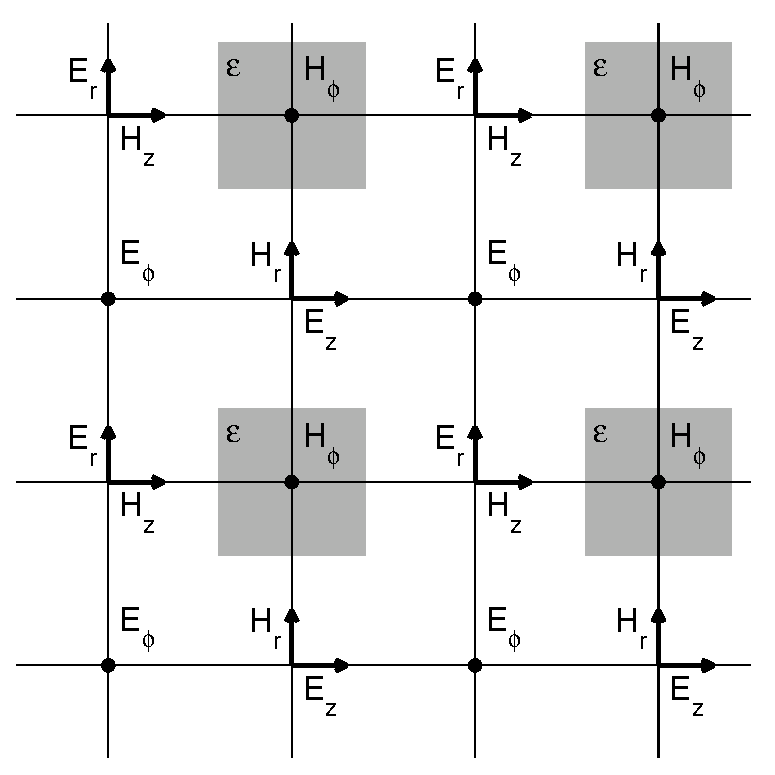
\includegraphics[width=7.8cm,clip=true]{Yee_bulk}
\end{figure}

The Yee lattice has the property that all the derivatives needed for
$\mathbf \nabla \times \mathbf H$ are known at the Yee lattice points of
$\mathbf E$.  For example, if you look at the $H_\phi$ location.
$\frac{dH_\phi}{dt}$ depends on $\frac{dE_r}{dz}$ and $\frac{dE_z}{dr}$.
This is great, because $E_r$ is known to the right and left of $H_\phi$,
and $E_z$ is known above and below $H_\phi$.

The same principle that the Yee lattice does with space, we also do with
time.  $\mathbf E$ and $\mathbf H$ are known at different times, so that
the time derivative of $\mathbf E$ is known at a $\mathbf H$ time and vice
versa.

\section{Maxwell's equations in cylindrical coordinates}

Here are Maxwell's equations in cylindrical coordinates.  We take the
fields to be of the form:
\begin{equation*}
\mathbf{E}(r,\phi,z) = \mathbf{E}_m(r,z)e^{i m \phi} 
\end{equation*}

Without further ado:
\begin{align}
\frac1c\frac{dH_r}{dt} &= \frac{dE_\phi}{dz} - \frac{im}r E_z\\
\frac1c\frac{dH_\phi}{dt} &= \frac{dE_z}{dr} - \frac{dE_r}{dz}\\
\frac1c\frac{dH_z}{dt} &= \frac{im}r E_r - \frac1r\frac{d(rE_\phi)}{dr}
\end{align}
\begin{align}
\frac\epsilon c\frac{dE_r}{dt} &= \frac{im}r H_z - \frac{dH_\phi}{dz} \\
\frac\epsilon c\frac{dE_\phi}{dt} &= \frac{dH_r}{dz} - \frac{dH_z}{dr} \\
\frac\epsilon c\frac{dE_z}{dt} &= \frac1r\frac{d(rH_\phi)}{dr} - \frac{im}r H_r
\end{align}


\chapter{PML}

PML (Perfectly Matched Layers) is used to provide absorbing boundary
conditions in either the $z$ or $r$ direction.  PML consists of a material
in which some of the field components are split into two fields, each of
which has a conductivity associated with it, which is responsible for the
absorption of the PML.

PML is a sort of material that contains a set of conductivities $\sigma_r$,
$\sigma_\phi$ and $\sigma_z$.  These conductivities are both $\mathbf{E}$
and $\mathbf{H}$ conductivities---yes, we have magnetic monopoles moving
around in our PML.  $\ddot\smile$ Each $\sigma$ causes absorption of
radiation in the direction it is named after.  Thus $\sigma_\phi$ is small,
and almost unnecesary, and is only needed because of the curvature of the
radial surface.  The value of $\sigma_\phi$ at a given radius is equal to
\begin{equation}
\sigma_\phi(r) = \frac1r \int_0^r \sigma_r(r)dr
\end{equation}

If we had a IDTD (Infinitesimal Difference Time Domain) code, PML would be
perfectly absorbing, regardless of the variation of $\sigma$ with position.
However, since meep is a lowly FDTD code, we have to make sure that
$\sigma$ varies only slowly from one grid point to the next.  We do this by
making $\sigma_z$ (for example) vary as $z^2$, with a maximum value of
$\sigma_{max}$ right in front of the boundary.  At the edge of the PML
region is a metalic boundary condition.  The optimal value of
$\sigma_{max}$ is determined by a tradeoff between reflection off the
metallic boundary, caused by too little a $\sigma_{max}$, and reflection
off the sigma itself, caused by too large a $\sigma_{max}$, which makes for
a large variation of $\sigma$ from one grid point to the next.

Here are the field equations for a PML material:
\begin{align}
\frac{dH_{r\phi}}{dt} &= - c \frac{im}r E_z             - \sigma_\phi H_{r\phi} &
\frac{dH_{rz}}{dt} &= c \frac{dE_\phi}{dz}              - \sigma_z H_{rz}\\
\frac{dH_{\phi z}}{dt} &= - c \frac{dE_r}{dz}           - \sigma_z H_{\phi z} &
\frac{dH_{\phi r}}{dt} &= c \frac{dE_z}{dr}             - \sigma_r H_{\phi r} \\
\frac{dH_{zr}}{dt} &= - c \frac1r\frac{d(rE_\phi)}{dr}  - \sigma_r H_{zr}  &
\frac{dH_{z\phi}}{dt} &= c \frac{im}r E_r               - \sigma_\phi H_{z\phi} \\
\epsilon\frac{dE_{r\phi}}{dt} &=   c \frac{im}r H_z             - \sigma_\phi E_{r\phi} &
\epsilon\frac{dE_{rz}}{dt} &= -c\frac{dH_\phi}{dz}              - \sigma_z E_{rz}\\
\epsilon\frac{dE_{\phi z}}{dt} &=   c \frac{dH_r}{dz}           - \sigma_z E_{\phi z} &
\epsilon\frac{dE_{\phi r}}{dt} &=-c \frac{dH_z}{dr}             - \sigma_r E_{\phi r} \\
\epsilon\frac{dE_{zr}}{dt} &=   c \frac1r\frac{d(rH_\phi)}{dr}  - \sigma_r E_{zr}  &
\epsilon\frac{dE_{z\phi}}{dt} &=-c \frac{im}r H_r               - \sigma_\phi E_{z\phi} 
\end{align}

\chapter{Of polaritons and plasmons}\label{polaritons}

Most real materials, at least in some frequency range, have polarizations
that are not actually instantaneously proportional to the local electric
field.  We model these polaritonic and plasmonic effects by introducing one
or more additional polarization fields, to be propogated along with the
electric and magnetic field.  The polarization field, $\mathbf{P}$, is a
vector field which exists on the electric field Yee lattice points.

The polarization field obeys a second order differential equation, which
means that we need to keep track of the polarization at two time steps, in
order to integrate it.

\begin{equation}
\frac{d^2\mathbf{P}}{dt^2} + \gamma \frac{d\mathbf{P}}{dt}
+ \omega^2 \mathbf{P} = \Delta\epsilon\ \omega^2 \mathbf{E}
\end{equation}

To this, we need add one more term to maxwell's equation for $\mathbf E$:

\begin{equation}
c \nabla \times \mathbf{H} = \epsilon_\infty \frac{d\mathbf{E}}{dt}
 + \frac{d\mathbf{P}}{dt}
\end{equation}

So far, the polarization is beautifully simple.  However, we would love to
be able to put polaritonic materials into our PML regions, and
unfortunately in the PML region the electric field has been split into two
components, so we need to figure out which of the two components gets the
contribution from $\frac{d\mathbf{P}}{dt}$.  The obvious solution to this
(well, maybe not exactly obvious, but it is the solution) is to split the
polarization field also into two components in the PML region, just as we
split the electric and magnetic fields.

The electric field propogation equations in PML then become:
\begin{align}
\epsilon\frac{dE_{r\phi}}{dt} &=   c \frac{im}r H_z
             - \sigma_\phi E_{r\phi} - \frac{dP_{r\phi}}{dt} \\
\epsilon\frac{dE_{\phi z}}{dt} &=   c \frac{dH_r}{dz}
             - \sigma_z E_{\phi z} - \frac{dP_{\phi z}}{dt} \\
\epsilon\frac{dE_{zr}}{dt} &=   c \frac1r\frac{d(rH_\phi)}{dr}
             - \sigma_r E_{zr} - \frac{dP_{zr}}{dt}
\end{align}
\begin{align}
\epsilon\frac{dE_{rz}}{dt} &= -c\frac{dH_\phi}{dz}
             - \sigma_z E_{rz} - \frac{dP_{rz}}{dt}\\
\epsilon\frac{dE_{\phi r}}{dt} &=-c \frac{dH_z}{dr}
             - \sigma_r E_{\phi r} - \frac{dP_{\phi r}}{dt} \\
\epsilon\frac{dE_{z\phi}}{dt} &=-c \frac{im}r H_r \label{polariton_pml}
             - \sigma_\phi E_{z\phi} - \frac{dP_{z\phi}}{dt}
\end{align}

\chapter{Hints for writing finite difference time domain code}

(Or \emph{Things I forgot many times, so I wrote down so maybe I won't make
  the same mistake again.})

There is just one rule to remember when writing time domain code, and that
is (as Lefteris has repeatedly told me) ``Always know \emph{when} each
equation is evaluated.''  The trick, of course, lies in knowing how to
apply this rule, and remembering to actually apply it (and I think the
latter is perhaps harder than the former).

As an example, I'll convert a PML polariton equation into a finite
difference equation taken from equation~\ref{polariton_pml} of
chapter~\ref{polaritons}.
\begin{equation*}
\epsilon\frac{dE_{z\phi}}{dt} = -c \frac{im}r H_r
             - \sigma_\phi E_{z\phi} - \frac{dP_{z\phi}}{dt}
\end{equation*}
If we consider the $\mathbf{E}$ timesteps to be at times $n$, $n+1$ etc.,
then this equation needs to be evaluated at time $n+\frac12$.  This is no
problem for most of the terms, but it means that the $\sigma_\phi
E_{z\phi}$ term needs to be an average of its values at time $n$ and
$n+1$.  In short (taking $\Delta t$ to be unity)...
\begin{equation*}
\epsilon (E_{z\phi}^{n+1} - E_{z\phi}^n) = -c \frac{im}r H_r^{n+\frac12}
  - \sigma_\phi ( E_{z\phi}^{n+1} + E_{z\phi}^n) - (dP_{z\phi}^{n+1} - dP_{z\phi}^n)
\end{equation*}
Simplifying a tad gives
\begin{equation*}
E_{z\phi}^{n+1} - E_{z\phi}^n = \frac1{\epsilon + \frac12\sigma_\phi}
    \left(-c \frac{im}r H_r^{n+\frac12}
  - \sigma_\phi E_{z\phi}^n - (dP_{z\phi}^{n+1} - dP_{z\phi}^n)\right)
\end{equation*}
Basically, that is all there is to it.  You now have the equation to
determine $E_{z\phi}^{n+1}$ from $E_{z\phi}^n$, $\frac{im}r
H_r^{n+\frac12}$, $dP_{z\phi}^{n+1}$ and $dP_{z\phi}^n$.

\chapter{Tutorial}

\begin{comment}
/*
\end{comment}
\section{A simple 2D system.}
\begin{comment}
*/
\end{comment}

This example is intended to let you quickly get started using meep to run
a simple calculation.  As such, it will include within it the complete code
of the example itself.  Meep is a C++ library, so your control file is a
small C++ program.

At the beginning of your control file, you have to include the ``meep.h''
header and use the ``meep'' namespace...
\begin{verbatim}
#include <meep.hpp>
using namespace meep;
\end{verbatim}

Next we create a function to define epsilon.  This function accepts a
``vec'' argument, and returns a double, which is the value of epsilon.  For
this example, we use an index-guided waveguide with some air slits cut in
it.  You can choose whatever units you like in which to define your
structure.  In this case we choose the width of the waveguide as our unit,
which is also equal to 1 micron.

\begin{verbatim}
const double half_cavity_width = 0.5*0.68, air_slit_width = 0.38,
             grating_periodicity = 0.48,
             half_waveguide_width = 1.0,
             num_air_slits = 15.0,
             high_dielectric = 12.0, low_dielectric = 11.5;
const double pml_thickness = 1.0;
const double x_center = 7.7 + pml_thickness;
const double y_center = 10.5 + pml_thickness;
double eps(const vec &rr) {
  // Displacement from center of cavity is r:
  const vec r = rr - vec(x_center, y_center);
  // First the air slits:
  double dx = fabs(r.x()) - half_cavity_width;
  if (dx < num_air_slits*grating_periodicity && dx > 0.0) {
    while (dx > grating_periodicity) dx -= grating_periodicity;
    if (dx < air_slit_width) return 1.0;
  }
  // Now check if the y value is within the waveguide:
  if (fabs(r.y()) < half_waveguide_width) return high_dielectric;
  // Otherwise we must be in the surrounding low dielectric:
  return low_dielectric;
}
\end{verbatim}
\begin{figure}
\label{simple_figure}
\caption{$E_z$}
\begin{center}
\includegraphics[width=4.8cm,clip=true]{simple-out/ez-000200-00}
\end{center}
\end{figure}
The main function should always start by creating an initialize object.
This object is responsible for setting up MPI if we are running on multiple
processors, and cleaning up properly when it is deleted (which means we are
done).
\begin{verbatim}
int main(int argc, char *argv[]) {
  initialize mpi(argc, argv);
\end{verbatim}
The ``s'' structure defines the contents of the unit cell.  It needs a
volume, which includes the size of the grid and the resolution, as well as
the epsilon function we defined earlier.  Here we also choose to use PML
absorbing boundary conditions in all directions, since we are interested in
the high Q mode in the cavity.
\begin{verbatim}
  const double amicron = 10; // a micron is this many grid points.
  const volume vol = voltwo(2*x_center, 2*y_center, amicron);
  const symmetry S = mirror(Y, vol) + rotate2(Y, vol);
  structure s(vol, eps, pml(pml_thickness), S);
\end{verbatim}
To avoid clutter, we'll create a directory to hold the output.  The
function \verb!make_output_directory! creates a directory based on the name
of the example program along with an extension.  It also backs up the C++
source file if it can find it.  If the directory already exists, then it
reuses it, unless the C++ control file has changed, in which case it
creates a new one.
\begin{verbatim}
  const char *dirname = make_output_directory(__FILE__);
  s.set_output_directory(dirname);
\end{verbatim}
The structure only holds the epsilon.  We will also need a ``fields''
object to hold our electric and magnetic fields.  We add a point source
oriented in the $E_z$ direction, located in the center of our cavity.
\begin{verbatim}
  fields f(&s);
  const double wavelength = 1.72;
  const double freq = 1.0/wavelength;
  f.add_point_source(Hy, freq, 10.0, 0.0, 5.0, vec(x_center,y_center));
\end{verbatim}
I'm not interested in seeing the source itself, so I'll keep time stepping
until the current time is greater than the last time at which the source is
running.
\begin{verbatim}
  while (f.time() < f.last_source_time()) f.step();
\end{verbatim}
Now we'll wait a bit (to let the low-Q modes die off) and then take a
snapshot of the fields in encapsulated postscript format.
\begin{verbatim}
  while (f.time() < 200.0) f.step();
  f.eps_slices();
\end{verbatim}
And now we're done, although you might wonder if we've done anything
worthwhile, since all we got out of this was a picture... All that is left
is (as a matter of principle) to delete the string containing the directory
name of our output directory.
\begin{verbatim}
  delete[] dirname;
}
\end{verbatim}

\begin{comment}
/*
\end{comment}
\section{A considerably more complicated 2D example.}
\begin{comment}
*/
\end{comment}

This example demonstrates a lot more of what you can do using dactyl.  The
system is the same as in the previous example, but this time we will
calculate the quality factor of the cavity.  Again, the entire control file
will be included here, but I'll skip over sections that have already been
explained.

\begin{verbatim}
#include "meep.h"

const double half_cavity_width = 0.5*0.68, air_slit_width = 0.38,
             grating_periodicity = 0.48,
             half_waveguide_width = 1.0,
             num_air_slits = 15.0,
             high_dielectric = 12.0, low_dielectric = 11.5;
const double pml_thickness = 1.0;
const double x_center = 7.7 + pml_thickness;
const double y_center = 10.5 + pml_thickness;
double eps(const vec &rr) {
  // Displacement from center of cavity is r:
  const vec r = rr - vec2d(x_center, y_center);
  // First the air slits:
  double dx = fabs(r.x()) - half_cavity_width;
  if (dx < num_air_slits*grating_periodicity && dx > 0.0) {
    while (dx > grating_periodicity) dx -= grating_periodicity;
    if (dx < air_slit_width) return 1.0;
  }
  // Now check if the y value is within the waveguide:
  if (fabs(r.y()) < half_waveguide_width) return high_dielectric;
  // Otherwise we must be in the surrounding low dielectric:
  return low_dielectric;
}
\end{verbatim}
This time we use the \verb!deal_with_ctrl_c();! function.  This is a handy
utility function that is useful when running your dactyl code
interactively.  It traps the SIGINT signal, so when you hit cntl-C, rather
than simply exiting, the global variable \verb!interrupt! is incremented.
If you really want to exit, just hit cntl-C again, and when
\verb!interrupt! reaches 2, the program will exit.
\begin{verbatim}
int main(int argc, char *argv[]) {
  initialize mpi(argc, argv);
  deal_with_ctrl_c();
  const double amicron = 10; // a micron is this many grid points.
  const volume vol = voltwo(2*x_center, 2*y_center, amicron);
  const symmetry S = mirror(Y, vol) + rotate2(Y, vol);
  mat ma(vol, eps, 0, S);
  ma.use_pml_everywhere(pml_thickness);
  const char *dirname = make_output_directory(argv[0]);
  ma.set_output_directory(dirname);
  fields f(&ma);
  const double wavelength = 1.72;
  const double freq = 1.0/wavelength;
  f.add_point_source(Hy, freq, 5.0, 0.0, 5.0, vec2d(x_center,y_center));
  f.use_metal_everywhere();
\end{verbatim}
We add an additional check below ``\verb!&& !interrupt!'' so that when the
user hits cntl-C we exit the loop.
\begin{verbatim}
  while (f.time() < f.find_last_source() && !interrupt) f.step();
  f.eps_slices();
  while (f.time() < 400.0 && !interrupt) f.step();
\end{verbatim}
This time we're going to run the simulation longer, so we would like to get
occasional informative messages.  To do this we define a variable to hold
the next time we want to print a message.
\begin{verbatim}
  double next_print_time = 500.0;
\end{verbatim}
To calculate the $Q$ of our cavity, we use a monitor point \verb!p!.  We
also store the value of $H_y$ at our monitor point in a file named ``hy''
periodically.  We create this file using \verb!create_output_file!, which
creates and opens a file for writing in the given output directory.  This
utility function works properly whether we are running in parallel or not.
\begin{verbatim}
  monitor_point *p = NULL;
  file *myout = create_output_file(dirname, "hy");
  while (f.time() <= 2000.0 && !interrupt) {
    // Now we'll start taking data!
    f.step();
\end{verbatim}
To get the monitor point data we use the \verb!get_new_point! method of
\verb!fields!.  This ends up creating a linked list containing the values
of the field at the monitor point as a function of time, which we will
later use to run harminv and get the $Q$.
\begin{verbatim}
    p = f.get_new_point(vec2d(x_center,y_center), p);
\end{verbatim}
We use the \verb!get_component! method to extract the (complex) fields from
the monitor point so we can print them.  We use the \verb!master_fprintf!
function because we only want to get one copy of the information even if
we're running in parallel.
\begin{verbatim}
    master_fprintf(myout, "%lg\t%lg\t%lg\n", f.time(),
                   real(p->get_component(Hy)),
                   imag(p->get_component(Hy)));
\end{verbatim}
Every time we reach the \verb!next_print_time! we print out a copy of the
slices, along with a little message indicating the time and the total
energy (which should be decaying at this point).  The function
\verb!master_printf! is a utility function that works basically like
\verb!printf!, except that when running in parallel only one of the
processors (the ``master'') does the printing.  You should use this
function rather than something like
``\verb!if (my_rank()==0) printf(...)!'', since the latter can cause
problems if the arguments to printf require synchronization between the
processes.
\begin{verbatim}
    if (f.time() >= next_print_time) {
      f.eps_slices();
      master_printf("Energy is %lg at time %lg\n",
                    f.total_energy(), f.time());
      next_print_time += 500.0;
    }
  }
\end{verbatim}
Files which are opened with \verb!create_output_file! need to be closed
with \verb!everyone_close!, which does the Right Thing when running in
parallel.
\begin{verbatim}
  everyone_close(myout);
\end{verbatim}
Having collected all the monitor point data, we now want to run
harminv\footnote{If you don't know what harminv is, I'm not going to
explain it here, so you may as well ask me in person (or even better, ask
Steven...} on it to find the $Q$ of our resonant cavity.  The
\verb!harminv! method gives us the complex amplitudes, the frequencies and
the decay rates.  The decay rate is given in the same units as the
frequency, so you could choose to view it as the imaginary part of the
frequency if you like.

This harminv step is the real reason for using the ctrl-C trick, since if
while running this example we get impatient and decide we have enough data
we can just hit ctrl-C and get the results using what data we have.  This
means you can just set the code to run for an excessively long time without
risking losing everything if you lose patience.
\begin{figure}
\label{complicated_figure}
\begin{center}
\fbox{\parbox{4in}{
\caption{Contents of ``freqs'' file}
\input{complicated-out/freqs}}}
\end{center}
\end{figure}

In case you're wondering about the ``\verb!\begin{verbatim}!'', it's there
so I can easily include the output in this manual (see
Figure~\ref{complicated_figure}).
\begin{verbatim}
  complex<double> *amp;
  double *freqs, *decays;
  int num;
  
  file *myfreqs = create_output_file(dirname, "freqs");
  master_fprintf(myfreqs, "\\begin{verbatim}\n");
  master_printf("Harminving Hy...\n");
  interrupt = 0; // Harminv even if we were interrupted.
  p->harminv(Hy, &amp, &freqs, &decays, &num, 0.8*freq, 1.2*freq, 5);
  for (int i=0;i<num;i++) {
    master_fprintf(myfreqs, "%lg\t%lg\t%lg\t%lg\t%lg\n",
                   freqs[i], decays[i], -freqs[i]/decays[i],
                   real(amp[i]), imag(amp[i]));
  }
  master_fprintf(myfreqs, "%cend{verbatim}\n", '\\');
  everyone_close(myfreqs);
  delete[] dirname;
}
\end{verbatim}


\begin{comment}
/*
\end{comment}
\section{Baby's First Bandstructure}
\begin{comment}
*/
\end{comment}

\begin{comment}
#include <stdio.h>
#include <stdlib.h>
#include "dactyl.h"

double eps(const vec &) {
  return 1.0;
}
const int rad = 10;
const int ttot = 1500*rad;
\end{comment}

In this example we calculate the lowest four TE modes of a simple hollow
metallic waveguide of radius one.

\begin{verbatim}
int main(int argc, char *argv[]) {
  initialize(argc, argv);
  FILE *ban = fopen("bands", "w");
  mat ma(volcyl(1.0, 0.0, rad), eps);
  for (int m=0;m<3;m++) {
    for (double k=0.0; k<= 1.01; k += 0.25) {
      master_printf("Working on k of %g and m = %d with a=%d...\n",
                    k, m, rad);
      fields f(&ma, m);
      f.use_bloch(k);
\end{verbatim}

There are a few tricks you should know before you decide to go about
calculating a band structure.  One of the biggest problems in calculating a
band structure in a time domain code is that of exciting all the modes you
are interested in.  dactyl makes this easy with a couple of ``fields''
methods, \verb-initialize_with_n_te-, and \verb-initialize_with_n_tm-.
These initialize the field with the n lowest TE and TM modes respectively.

\begin{verbatim}
      f.initialize_with_n_te(4);
\end{verbatim}

The band structure code itself begins with a call to
\verb-prepare_for_bands-, which allocates space to store the field
data, which is later used for the band structure calculation.  Its third
argument is the maximum frequency you are interested in.

\begin{verbatim}
      double fmax = 1.0, qmin = 200;
      f.prepare_for_bands(0, ttot, fmax, qmin);
      for (int t=0;t<ttot;t++) {
\end{verbatim}

The second band structure function is \verb-record_bands-, which just
copies the fields into the already allocated arrays for future use.

\begin{verbatim}
        f.record_bands();
        f.step();
      }
\end{verbatim}

Finally, the band structure is actually computed and output by the method
\verb-output_bands-.  The key thing to know about
\verb-output_bands- is that its last argument should be something like
twice the number of modes which have a frequency below your maximum.
Rounding this number up slows the code down considerably, but can sometimes
fix problems where harminv (which is used internally) doesn't find the
modes correctly.  Usually, however, when harminv fails it means you are
misunderstanding something (for example, fmax may be less than the lowest
frequency mode).

\begin{verbatim}
      f.output_bands(ban, "band", 35);
    }
  }
  fclose(ban);
  finished();
}
\end{verbatim}


\begin{comment}
#include <stdio.h>
#include <stdlib.h>

#include <meep.h>
using namespace meep;

const int a = 10;
\end{comment}

\section{Computing the band structure of an omniguide}

In this section we give as an example of a more complicated band structure,
a computation of the band structure of an omniguide.  The output of this
program is shown in Figure~\ref{omniguidebands}.

\begin{verbatim}
const int num_layers = 3;
const double rcore = 3.0;

double guided_eps(const vec &v) {
  double rr = v.r() - rcore;
  if (rr > num_layers + 0.3) return 1.0; // outside the entire waveguide
  if (rr < 0.0) return 1.0;   // vacuum in the core
  while (rr > 1.0) rr -= 1.0; // calculate (r - rcore) % 1
  if (rr < 0.3) return 21.16; // in the high dielectric
  return 1.6*1.6;             // in the low dielectric
}
double vacuum_eps(const vec &v) { return 1.0; }
\end{verbatim}

\begin{comment}
int main(int argc, char **argv) {
  initialize mpi(argc, argv);
  deal_with_ctrl_c();
  printf("Running omniguide!\n");

  const double ttot = 1000.0;
  structure s(volcyl(rcore + num_layers + 0.3, 0.0, a), guided_eps);
  const char *dirname = make_output_directory(__FILE__);
\end{comment}

For this band structure example, we use the grace object to create our
plot.
\begin{verbatim}
  grace g("bands", dirname);
  g.set_range(0.0, 0.35, 0.0, 0.35);
\end{verbatim}
\begin{comment}
  s.set_output_directory(dirname);
  structure vac(&s);
  vac.set_epsilon(vacuum_eps);
\end{comment}

Since the m = 0 modes are pure TE or TM, it makes sense to calculate the
two polarizations separately.  Not only does this give us more interesting
output, but it doesn't cost us any time, to speak of, and actually makes
the band structure much easier to converge.  However, for brevity, I won't
include here in the manual computation of the TM modes, but will skip
straight to the TE modes.

\begin{comment}
  {
    const int m=0;
    g.new_set();
    g.set_legend("m = 0, TM");
    for (double k=0.0;k<0.356 && !interrupt;k+=0.05) {
      char k_and_m[10];
      snprintf(k_and_m, 10, "%g-%d", k, m);
      printf("Working on k of %g and m=0 TM with a=%d...\n", k, a);
      fields f(&vac, m);
      f.use_bloch(k);
      f.verbose(1);
      f.phase_in_material(&s, 1000);
      f.initialize_with_n_tm(9);
      double next_slice_time = 0.0;
      while (f.is_phasing() && !interrupt) f.step();
      f.prepare_for_bands(veccyl(4.801,0.0), ttot, .40, 300, 0.0);
      f.prepare_for_bands(veccyl(3.801,0.0), ttot, .40, 300, 0.0);
      f.prepare_for_bands(veccyl(3.301,0.0), ttot, .40, 300, 0.0);
      const double stoptime = f.time() + ttot;
      while (f.time() < stoptime && !interrupt) {
        f.record_bands();
        f.step();
      }
      f.grace_bands(&g, 40);
    }
  }
\end{comment}

\begin{figure}
\label{omniguidebands}
\caption{Omniguide band structure.}
\includegraphics[width=8.8cm,clip=true]{omniguide-out/bands}
\end{figure}

\begin{verbatim}
  for (int m=0;m<2 && !interrupt;m++) {
    g.new_set();
    char m_string[30];
    if (m) snprintf(m_string, 30, "m = %d", m);
    else snprintf(m_string, 30, "m = 0, TE");
    g.set_legend(m_string);
    for (double k=0.0;k<0.351 && !interrupt;k+=0.05) {
\end{verbatim}
In order to populate the modes that we are interested in, we first populate
the modes of an empty waveguide (whose modes are known), and then
adiabatically transform from that waveguide into our omniguide structure.
\begin{verbatim}
      printf("Working on k of %g and %s with a=%d...\n", k, m_string, a);
      fields f(&vac, m);
      f.use_bloch(k);
      f.verbose(1);
      f.phase_in_material(&s, 1000);
\end{verbatim}
We initialize the fields with both TE and TM modes, and then phase in the
epsilon as usual, and then do the actual phasing in of the structure.
\begin{verbatim}
      f.initialize_with_n_te(9);
      if (m) f.initialize_with_n_tm(9);
      while (f.is_phasing() && !interrupt) f.step();
\end{verbatim}
Again, the band structure code is pretty normal, with the only real
difference being that in this case we \emph{really} want to have specify a
large $Q_{min}$, to help meep to distinguish between real modes and
spurious noise.  Note that we are using metallic boundary conditions, so
all physical modes should have infinite lifetime.
\begin{verbatim}
      f.prepare_for_bands(veccyl(4.801,0.0), ttot, .35, 300, 0.0);
      f.prepare_for_bands(veccyl(1.801,0.0), ttot, .35, 300, 0.0);
      f.prepare_for_bands(veccyl(2.801,0.0), ttot, .35, 300, 0.0);
      const double stoptime = f.time() + ttot;
      while (f.time() < stoptime && !interrupt) {
        f.record_bands();
        f.step();
      }
\end{verbatim}
Finally, we just need to compute and output the bands.  We are careful here
to keep in mind that when $m > 0$, there are twice as many bands, since
there are both TM and TE modes.
\begin{verbatim}
      f.grace_bands(&g, m?80:40);
    }
\end{verbatim}
The band is actually printed to disk only when the grace object is
destroyed, which in this case happens just before the program exits.
\begin{comment}
  }
}
\end{comment}

\section{Band structure of a polariton}

\begin{comment}
#include <stdio.h>
#include <stdlib.h>
#include <signal.h>

#include "dactyl.h"

static int stopnow = 0;
void handle_control_c(int i) {
  printf("Be patient, I'll stop as soon as it's convenient...\n");
  stopnow = 1;
}

const double rmax = 1.0;
\end{comment}

Here we compute and plot the band structure of a polariton material.  We
look at a simple metallic waveguide filled with a polaritonic material.
The material we look at has an epsilon of 13.4 and a longitudinal phonon
frequency of 0.7 and a transverse phonon frequency of 0.4.

\begin{figure}
\label{polaritonbands}
\caption{Polariton band structure.}
\epsfig{file=polaritonbands.eps,width=7.8cm,angle=270}
\end{figure}

\begin{verbatim}
double eps(double r, double z) { return 13.4; }
double one(double r, double z) { return 1; }
\end{verbatim}

\begin{comment}
int main(int argc, char **argv) {
  signal(SIGINT, handle_control_c);
  const int rad = 10;
  const int m = 0;
  double k;
  const int ttot = 1000*rad;  
\end{comment}

\begin{comment}
  mat ma(eps, rmax, 0.0, rad);
  const char *dirname = make_output_directory(argv[0]);
  printf("Storing output in directory %s/\n", dirname);
  FILE *ban = create_output_file(dirname, "bands");
  ma.set_output_directory(dirname);
\end{comment}

To create the polaritonic material, we add the polarizability to the
material after we have created it.

\begin{verbatim}
  ma.add_polarizability(one, 0.4, 0.01, 27.63);//0.1);//
\end{verbatim}

In order to easily calculate the bandstructure, we start out with a simple
material with a material with the same epsilon and polarization
frequencies, but with no coupling between the phonons and the
electromagnetic fields.

\begin{verbatim}
  mat vac(&ma);
  vac.make_average_eps();
  vac.add_polarizability(one, 0.4, 0.01, 0.0);
  for (k=0.0;k<30.01 && !stopnow;k+=2.5) {
    printf("Working on k of %g and m = %d...\n", k, m);
    fields f(&vac, m);
    f.use_bloch(k);
\end{verbatim}

We will rather quickly move from this fake material to the actual
polaritonic material.

\begin{verbatim}
    f.phase_in_material(&ma, 10);
\end{verbatim}

Now we excite the first TE mode (we're only looking at m = 0 here), and
remember to excite along with it the phonon with which it couples.

\begin{verbatim}
    f.initialize_with_nth_te(1);
    f.initialize_polarizations();
\end{verbatim}

Finally, we compute the band structure as usual.

\begin{verbatim}
    while (f.is_phasing()) f.step();
    f.prepare_for_bands(0, ttot, .7+0.5*k/30.0, 30);
    
    for (int t=0; t < ttot+1 && !stopnow; t++) {
      f.record_bands();
      f.step();
    }
    f.output_bands(ban, "band", 16);
\end{verbatim}
\begin{comment}
    fflush(ban);
  }
  fclose(ban);
}
\end{comment}

The final output of this routine (as calculated using the ``plot'' program)
is shown in Figure~\ref{polaritonbands}.


\begin{comment}
#include <stdio.h>
#include <stdlib.h>
#include <signal.h>
\end{comment}

\section{Energy conservation in cylindrical coordinates}

In this example, we compute the total energy over time for a polaritonic
material in cylindrical coordinates.  Eventually I figure I may extend this
example to demonstrate energy/flux conservation using PML.  That would
definitely be more impressive.

\begin{figure}
\label{econs_cyl}
\caption{Energy vs. Time.}
\includegraphics[width=8.8cm,clip=true]{energy_cons-out/energy}
\end{figure}

\begin{comment}
#include "meep.h"

const double a = 10;
\end{comment}

For our example polaritonic material, we'll use an $\epsilon(0)$ of 13.4.
We will put the polaritons in just one quarter of our system to add a
little extra excitement.

\begin{verbatim}
double eps(const vec &) { return 13.4; }
double one(const vec &p) { return (p.z() > 15.0)?1:0; }
\end{verbatim}
\begin{comment}
int main(int argc, char **argv) {
  initialize mpi(argc, argv);
  deal_with_ctrl_c();
  const double ttot = 600.0;
\end{comment}
We use a long and skinny system so as to exaggerate any errors that may
crop up at small $r$.
\begin{verbatim}
  mat ma(volcyl(1.0,20.0, a), eps);
\end{verbatim}
\begin{comment}
  const char *dirname = make_output_directory(__FILE__);
  ma.set_output_directory(dirname);
  ma.add_polarizability(one, 0.25, 0.1, 3.0);
  fields f(&ma);
  grace g("energy", dirname);
\end{comment}
We use several point sources, to cover a broad frequency range, just for
the heck of it.
\begin{verbatim}
  f.add_point_source(Ep, 0.6 , 1.8, 0.0, 8.0, vec(0.5,2.0));
  f.add_point_source(Ep, 0.4 , 1.8, 0.0, 8.0, vec(0.5,2.0));
  f.add_point_source(Ep, 0.33, 1.8, 0.0, 8.0, vec(0.5,2.0));
\end{verbatim}
\begin{comment}
  double next_printtime = 50;
  while (f.time() < ttot && !interrupt) {
    if (f.time() >= next_printtime) {
      next_printtime += 50;
      master_printf("Working on time %lg...  ", f.time());
      master_printf("energy is %lg\n", f.total_energy());
\end{comment}
We plot the total energy, the electromagnetic energy and the
``thermodynamic energy'' which is the energy that is either stored in the
polarization, or has been converted into heat, or (if we had a saturating
gain system) perhaps is stored in a population inversion.
\begin{verbatim}
      g.output_out_of_order(0, f.time(), f.total_energy());
      g.output_out_of_order(1, f.time(), f.field_energy_in_box(f.v.surroundings()));
      g.output_out_of_order(2, f.time(), f.thermo_energy_in_box(f.v.surroundings()));
\end{verbatim}
\begin{comment}
    }
    f.step();
  }
}
\end{comment}



\begin{comment}
#include <stdio.h>
#include <stdlib.h>
#include <signal.h>
\end{comment}

\section{Energy conservation in one dimension}

In this example, we compute the total energy over time for a polaritonic
material in one dimension to verify that it is indeed conserved.  This also
demostrates the support for 1D systems.

\begin{figure}
\label{econs_1d}
\caption{Energy vs. Time.}
\epsfig{file=energy_cons_1d-out/energy.eps,width=8.8cm}
\end{figure}

To begin with, to use a 1D system, we include ``tidod.h'' rather than
``dactyl.h.''  ``tidod'' stands for TIme Domain One Dimensional.  

\begin{verbatim}
#include "tidod.h"

const int rad = 10;
\end{verbatim}

For our example polaritonic material, we'll use an $\epsilon(0)$ of 13.4.

\begin{verbatim}
double eps(double z) { return 13.4; }
double one(double z) { return 1; }
\end{verbatim}
\begin{comment}
int main(int argc, char **argv) {
  deal_with_ctrl_c();
  const double ttot = 600.0;
\end{comment}
In various places we will need to add a ``\verb!_1d!'' as we make the
change from a cylindrical system to a 1D system.
\begin{verbatim}
  mat_1d ma(eps, 10.0, rad);
\end{verbatim}
\begin{comment}
  const char *dirname = make_output_directory(argv[0]);
  ma.set_output_directory(dirname);
\end{comment}
The polarizability is added as usual...
\begin{verbatim}
  ma.add_polarizability(one, 0.25, 0.01, 3.0);
  fields_1d f(&ma);
  grace g("energy", dirname);
\end{verbatim}
We use several plane wave sources, to cover a broad frequency range, just
for the heck of it.
\begin{verbatim}
  f.add_source(Ex, 0.6 , 0.8, 0.0, 8.0, 2.0);
  f.add_source(Ex, 0.4 , 0.8, 0.0, 8.0, 2.0);
  f.add_source(Ex, 0.33, 0.8, 0.0, 8.0, 2.0);
\end{verbatim}
\begin{comment}
  double next_printtime = 10;
  while (f.time() < ttot && !interrupt) {
    if (f.time() >= next_printtime) {
      next_printtime += 10;
      printf("Working on time %lg...  ", f.time());
      printf("energy is %lg\n", f.total_energy());
\end{comment}
We plot the total energy, the electromagnetic energy and the
``thermodynamic energy'' which is the energy that is either stored in the
polarization, or has been converted into heat, or (if we had a saturating
gain system) perhaps is stored in a population inversion.
\begin{verbatim}
      g.output_out_of_order(0, f.time(), f.total_energy());
      g.output_out_of_order(1, f.time(),
                            f.electric_energy_in_box(0.0,10.0)
                          + f.magnetic_energy_in_box(0.0,10.0));
      g.output_out_of_order(2, f.time(),
                            f.thermo_energy_in_box(0.0,10.0));
\end{verbatim}
\begin{comment}
    }
    f.step();
  }
}
\end{comment}



\begin{comment}
#include <stdio.h>
#include <stdlib.h>
#include <signal.h>

#include "dactyl.h"
\end{comment}

\section{Epsilon of a polaritonic material in one dimension}

In this example, we compute epsilon as a function of frequency for a simple
polaritonic material.  This example is done in one dimension for speed
purposes.

One thing to be aware of when using polaritonic materials, is that
generally you will be needing a rather higher grid resolution than you may
be used to in order to properly model the material.  Here I am using an $a$
of just 20, and if you look at figure~\ref{epsilon_polariton}, you can see
that the curve deviates significantly from the predicted result, which
would be essentially symmetric around the resonant frequency of $0.4$.

\begin{figure}
\label{epsilon_polariton}
\caption{Epsilon of a polaritonic material.}
\epsfig{file=epsilon_polariton_1d-out/eps.eps,width=8.8cm}
\end{figure}


\begin{comment}
const double rmax  = 2.0;
const double a = 20;
const double pml_thickness = 2.0;
const double zsize = 4/a + 2*pml_thickness;
\end{verbatim}

For our example polaritonic material, we'll use an $\epsilon(0)$ of 13.4.

\begin{verbatim}
double eps(const vec &) { return 13.4; }
\end{verbatim}
\begin{comment}
double one(const vec &) { return 1; }

int main(int argc, char **argv) {
  deal_with_ctrl_c();
  const double ttot = 600.0;
  mat ma(volone(zsize, a), eps);
  const char *dirname = make_output_directory(argv[0]);
  printf("Storing output in directory %s/\n", dirname);
  ma.set_output_directory(dirname);
\end{comment}
Notice that the polaritonic material will be within the PML.  This is fine.
Polaritons and PML are friends.
\begin{verbatim}
  ma.use_pml_right(pml_thickness);
  ma.use_pml_left(pml_thickness);
  ma.add_polarizability(one, 0.4, 0.01, 27.63);
\end{verbatim}
\begin{comment}
  fields f(&ma);
  double sourceloc = pml_thickness+1.0/(double)a;
\end{comment}
We use a single rather high frequency (and very broad) plane wave source,
to cover a broad frequency range.  For a plane source in 1D we don't really
need a source profile.
\begin{verbatim}
  f.add_plane_source(0.9 , 0.8, 0.0, 8.0, one, vec(sourceloc));
\end{verbatim}
We use a couple of monitor points to determine epsilon.
\begin{verbatim}
  monitor_point *left = NULL, *right = NULL;
\end{verbatim}
\begin{comment}
  double next_printtime = 50;
  while (f.time() < ttot && !interrupt) {
    if (f.time() >= next_printtime) {
      next_printtime += 50;
      printf("Working on time %lg...  ", f.time());
      printf("energy is %lg\n", f.field_energy());
    }
\end{comment}
The monitor points are located one grid spacing from one another.  The
\verb*|get_new_point| method appends the fields at a given time to a
monitor point linked list.
\begin{verbatim}
    left  = f.get_new_point(vec(sourceloc+1.0/a), left );
    right = f.get_new_point(vec(sourceloc+2.0/a), right);
\end{verbatim}
\begin{comment}
    f.step();
  }
  grace g("eps", dirname);
  complex<double> *al, *ar, *freqs;
  int numl, numr;
  printf("Working on left fourier transform...\n");
\end{comment}
When the time stepping is over, we take a fourier transform of the fields
at the two monitor points.
\begin{verbatim}
  left->fourier_transform(Ex, &al, &freqs, &numl, 0.301, 0.5, 1000);
\end{verbatim}
\begin{comment}
  delete[] freqs;
  printf("Working on right fourier transform...\n");
  right->fourier_transform(Ex, &ar, &freqs, &numr, 0.301, 0.5, 1000);
  if (numl != numr) printf("Aaack you need both nums to be the same!\n");
  g.new_set();
  g.set_legend("\\x\\e\\s2\\N");
\end{comment}
Finally we calculate the complex index of refraction using the equation
\begin{equation*}
i \omega \Delta x n(\omega) = \log \left(\frac{E'(\omega)}{E(\omega)}\right)
\end{equation*}
\begin{verbatim}
  for (int i=0;i<numl;i++) {
    complex<double> I = complex<double>(0,1);
    complex<double> n = (log(ar[i]/al[i]))/(I*(1.0/a)*2*pi*freqs[i]);
    g.output_point(real(freqs[i]), real(n*n));
  }
\end{verbatim}
\begin{comment}
  g.new_set();
  g.set_legend("\\x\\e\\s2\\N");
  for (int i=0;i<numl;i++) {
    complex<double> I = complex<double>(0,1);
    complex<double> n = (log(ar[i]/al[i]))/(I*(1.0/a)*2*pi*freqs[i]);
    g.output_point(real(freqs[i]), imag(n*n));
  }
}
\end{comment}



\section{Dielectric function of a material with loss and gain}

\begin{comment}
#include <stdio.h>
#include <stdlib.h>
#include <signal.h>

#include "dactyl.h"

const int rad = 10;
const int m = 0;
const double eps_value = 2.25;
const double fmin = 0.05;

const double pml = 1.0;
const int npml = (int)(0.5+pml*rad);
const double zsize = 2*pml+10/(double)rad;//+1.0/freq;
const double rmax  = 6/(double)rad;
const double zmiddle = zsize/2;
const double sourceloc = zmiddle - 4/(double)rad;

const double r_look = 1.5/rad, z_look = zmiddle, d = 1.0/rad;

complex<double> source_sharp(double r) {
  double sig = 1.0/rad;
  double dr = r - rmax*.5;
  if (fabs(r) >= rmax) return 0.0;
  return exp(-dr*dr/(2*sig*sig))/sqrt(sig);
}
double eps(double r, double z) { return eps_value; }
double one_in_middle(double r, double z) {
  const double midmax = r_look+2.0/(double)rad;
  const double midwid = 2/(double)rad;
  if (r <= midmax && z >= zmiddle-midwid && z < zmiddle+midwid) {
    return 1;
  } else {
    return 0;
  }
}

int main(int argc, char **argv) {
  deal_with_ctrl_c();
  const char *dirname = make_output_directory(argv[0]);
  printf("Using pml of %lg thickness.\n", pml);
  printf("Using an rmax of %lg\n", rmax);
  mat ma(eps, rmax + pml, zsize, rad);
  printf("I expect %g reflection off pml\n", ma.use_pml(pml,pml,fmin));
  ma.set_output_directory(dirname);
\end{comment}

In this section, we demonstrate a better way to calculate the dielectric
function, and illustrate it by computing the dielectric function of a
material with a normal lossy resonance as well as a gain line.  Gain in the
PML is a bad idea, so we restrict the polarizabilities to exist only in the
middle of the system (which is surrounded by PML).

\begin{figure}
\label{lossgain_epsilon}
\caption{Dielectric function of a material with loss and gain.}
\epsfig{file=lossgain_epsilon-out/eps.eps,width=8.8cm}
\end{figure}

\begin{verbatim}
  ma.add_polarizability(one_in_middle, 0.195, 0.03, 0.25*.25/.195);
  ma.add_polarizability(one_in_middle, 0.25, 0.03,-0.25);
\end{verbatim}

\begin{comment}
  ma.output_slices();

  fields f(&ma, m);
\end{comment}

For sources, we use a series of broad point sources covering the frequency
range of interest.

\begin{verbatim}
  f.add_source(Ep, 0.13, 0.8, 0.0, 8.0, sourceloc+0.0, source_sharp);
  f.add_source(Ep, 0.21, 0.8, 0.0, 8.0, sourceloc+0.0, source_sharp);
  f.add_source(Ep, 0.3 , 0.8, 0.0, 8.0, sourceloc+0.0, source_sharp);
  f.add_source(Ep, 0.43, 0.8, 0.0, 8.0, sourceloc+0.0, source_sharp);
\end{verbatim}
\begin{comment}
  printf("Working with a=%d...\n", rad);
  monitor_point *left = NULL, *right = NULL, *middle = NULL,
                *top = NULL, *bottom = NULL;
  double next_printtime = 10;
  while (f.time() < 110 && !interrupt) {
    if (f.time() >= next_printtime) {
      next_printtime += 10;
      printf("Working on time %lg...  ", f.time());
      printf("energy is %lg\n", f.total_energy());
      if (f.time() > -90) f.output_slices();
    }
    f.step();
\end{comment}

The calculation proceeds as usual, except that we now keep track of a set
of monitor points that will allow us to take a laplacian of the $H_z$ field
component.  We choose $m=0$, so we won't have to deal with the $\phi$
derivative.

\begin{verbatim}
    left   = f.get_new_point(r_look    , z_look - d, left);
    middle = f.get_new_point(r_look    , z_look    , middle);
    top    = f.get_new_point(r_look + d, z_look    , top);
    bottom = f.get_new_point(r_look - d, z_look    , bottom);
    right  = f.get_new_point(r_look    , z_look + d, right);
\end{verbatim}
\begin{comment}
  }

  grace g("eps", dirname);
  complex<double> *al, *ar, *am, *at, *ab, *freqs;
  int numl, numr;
  printf("Working on left fourier transform...\n");
\end{comment}

We fourier transform $H_z$ at each point:

\begin{verbatim}
  left->fourier_transform(Hz, &al, &freqs, &numl, 0.101, 0.5, 1000);
\end{verbatim}
\begin{comment}
  delete[] freqs;
  printf("Working on middle fourier transform...\n");
  middle->fourier_transform(Hz, &am, &freqs, &numr, 0.101, 0.5, 1000);
  delete[] freqs;
  printf("Working on top fourier transform...\n");
  top->fourier_transform(Hz, &at, &freqs, &numr, 0.101, 0.5, 1000);
  delete[] freqs;
  printf("Working on bottom fourier transform...\n");
  bottom->fourier_transform(Hz, &ab, &freqs, &numr, 0.101, 0.5, 1000);
  delete[] freqs;
  printf("Working on right fourier transform...\n");
  right->fourier_transform(Hz, &ar, &freqs, &numr, 0.101, 0.5, 1000);
  if (numl != numr) printf("Aaack you need both nums to be the same!\n");
  g.new_set();
  g.set_legend("\\x\\e\\s1\\N");
  complex<double> *epsilon = new complex<double>[numl];
\end{comment}

Finally, we calculate the laplacian of $H_z(\omega)$, which is equal to
$-k^2 H_z(\omega)$, from which we extract epsilon.

\begin{verbatim}
  for (int i=0;i<numl;i++) {
    complex<double> ksqr = -(ar[i]+al[i]-2*am[i]
                             + at[i]+ab[i]-2*am[i]
                             + (at[i]-ab[i])/2/r_look/rad
                             )*rad*rad/am[i];
    epsilon[i] = ksqr/freqs[i]/freqs[i]/(2*pi*2*pi);
  }
\end{verbatim}

I've left out the bulk of this example from the manual itself, since it
is pretty much the same as the previous examples.  Among other features, we
use the grace functions to plot the result, which can be seen in
Figure~\ref{lossgain_epsilon}.

\begin{comment}
  for (int i=0;i<numl;i++) {
    g.output_point(real(freqs[i]), real(epsilon[i]));
  }
  g.new_set();
  g.set_legend("\\x\\e\\s2\\N");
  for (int i=0;i<numl;i++) {
    g.output_point(real(freqs[i]), imag(epsilon[i]));
  }
}
\end{comment}


\section{Nonlinear materials}

FIXME: Add a nice discussion of nonlinear materials here...

In this example, we will use a CW source and compute the amplitude of the
field at a given position and time as a function of the source amplitude.
The result will be linear as long as the material remains in the linear
regime.  Once we have departed from the linear regime, we get more
complicated behavior.  Yes, this is a stupid example...

\begin{figure}
\label{nonlinear_field_shape}
\caption{Field vs. source amplitude with nonlinear material}
\includegraphics[width=14cm,clip=true]{nonlinear-out/ez-000400-00}
\end{figure}

The system is shown in Figure~\ref{nonlinear_field_shape}.  It is a 2D
metallic waveguide with vacuum $\epsilon$ of 2.25.  In the center of the
cell is a small region that is linear which contains the source, and the
rest of the waveguide contains a nonlinear material.  Both ends of the
waveguide have PML absorbing boundary conditions.

\begin{comment}
#include <stdio.h>
#include <stdlib.h>
#include <signal.h>

#include <meep.hpp>
using namespace meep;

const double a = 10.0;
const int m = 0;
const double eps_value = 2.25;

const double pml_thickness = 2.0;
const double xmax = 60.0;
const double ymax = 1.0;

double eps(const vec &v) {
  return eps_value;
}
\end{comment}
\begin{verbatim}
const double alpha_value = 0.07;
double alpha(const vec &v) {
  if (fabs(v.x() - xmax/2.0) < .51) return 0.0;
  return alpha_value;
}
\end{verbatim}

\begin{comment}
int main(int argc, char **argv) {
  initialize mpi(argc, argv);
  deal_with_ctrl_c();
  const char *dirname = make_output_directory(__FILE__);
  grid_volume v = vol2d(xmax, ymax, a);
  const symmetry S = mirror(X,v) + mirror(Y,v);
  structure s(v, eps, pml(pml_thickness, X), S);
  s.set_output_directory(dirname);
  grace g("field", dirname);
  g.output_point(0.0, 0.0);
  g.output_point(0.0, 0.0);
\end{comment}

The set\_chi3 method is used to set the chi3 coefficient.

\begin{verbatim}
  s.set_chi3(alpha);
\end{verbatim}

We use a CW source at a frequency of 0.4, which gives single-mode behavior
when the amplitude is small.  Also note that we use real fields, since
complex fields are incorrect for nonlinear materials.

\begin{verbatim}
  continuous_src_time my_source(0.4,  0.8);
  for (double amp = 0.05; amp <= 1.01 && !interrupt; amp += 0.01) {
    fields f(&s, m);
    f.use_real_fields();
    f.add_point_source(Ez, my_source, vec(xmax*0.5,ymax*0.5), amp);
\end{verbatim}

\begin{figure}
\label{nonlinear_field}
\caption{Field vs. source amplitude with nonlinear material}
\includegraphics[width=8.8cm,clip=true]{nonlinear-out/field}
\end{figure}

Time stepping, etc, is done as usual.  We monitor the field at one end of
the cell, which gives Figure~\ref{nonlinear_field}, which show the field
versus source amplitude.

\begin{comment}
    master_printf("Working with A=%g...\n", amp);
    double next_printtime = 400;
    while (f.time() < 10.1*xmax && !interrupt) {
      if (f.time() >= next_printtime) {
        next_printtime += 100;
        //master_printf("Working on time %g...  ", f.time());
        //master_printf("energy is %g\n", f.field_energy());
	f.output_hdf5(Ez, f.total_volume());
      }
      f.step();
    }
    g.output_point(amp, real(f.get_field(Ez,vec(1.2*pml_thickness,ymax/2))));
  }
}
\end{comment}


\appendix

\input{gpl.tex}

\end{document}
